%
% Angepasste FOM Seminarvorlage
%
\documentclass[12pt,a4paper,listof=totoc,bibliography=totoc]{scrartcl}

\usepackage[english]{babel}			% englische Namen/Umlaute
\usepackage[utf8]{inputenc}	    	% Zeichensatzkodierung
\usepackage{silence}
 \WarningFilter{scrartcl}{Usage of package `fancyhdr'}
 \WarningFilter{scrartcl}{Usage of package `parskip'}
\usepackage{fancyhdr}
\usepackage{graphicx}               % Einbinden von Bildern
\usepackage[hidelinks]{hyperref}	% Klickbare Verweise und \autoref{label}
\usepackage[intoc]{nomencl}
\usepackage{setspace}
\usepackage{parskip}
\usepackage{caption}
\usepackage{float}
\usepackage{listings}
\usepackage{scrhack}
\usepackage{geometry}
 \geometry{a4paper, left=40mm, right=20mm, top=40mm, bottom=20mm}
\renewcommand{\familydefault}{\sfdefault}
\renewcommand{\ttdefault}{pcr}
\renewcommand{\lstlistlistingname}{Listings}
\renewcommand{\lstlistingname}{Listing}
\usepackage{float}
\floatstyle{plaintop}
\restylefloat{table}

% Bildueberschrift oben und rechtsbuendig
\captionsetup{labelfont=bf, textfont=bf}
\captionsetup{justification=raggedright,singlelinecheck=false}

% Blocksatz
\def\justify{%
  \rightskip=0pt
  \spaceskip=0pt
  \xspaceskip=0pt
  \relax
}

%
%	Hier werden Titel, Bearbeiter und das Datum eingetragen
%
\newcommand\svthema{Digitales Live Studium}
\newcommand\svperson{Christian Frank (\#473088)}
\newcommand\svdatum{\today}
\newcommand\lvname{Projekt \& Innovation}
\newcommand\lvtyp{Sommerkonferenz Sopron 2025}
\newcommand\lvinst{FOM - Hochschule für Oekonomie \& Management}
\newcommand\lvbetr{Prof. Dr. Benjamin Niestroj}

\hypersetup{ % Thema und Author in die Meta-Daten der PDF
  pdftitle={\svthema}, 
  pdfauthor={Christian Frank},
  pdfsubject={Digitales Live Studium},
  pdfkeywords={FOM, DLS, BMI, Education}
}

\begin{document}

% Titel
\title{ \huge\textbf{\svthema} }
\author{ {\svperson} \\ \svdatum }
\date{ \normalsize \centering 
\includegraphics[width=0.3\textwidth]{FOM}\\ {\lvname} \\ {\lvbetr} \\ {\lvinst} \\ {\lvtyp} }

% Seitennummer oben
\pagestyle{fancy}
\fancyhf{}
\fancyhf[ch]{\thepage}
\renewcommand\headrulewidth{0pt}

\maketitle
\thispagestyle{empty} % laesst die Seitennummer auf der Titelseite verschwinden
\pagenumbering{Roman}

\begin{abstract}
In this paper, we will examine the Business Model Innovation that led FOM to develop the digital live format in the aftermath of the COVID-19 pandemic. We will also look at the actions of other players in the secondary education market.

\end{abstract}

\vfill
\begin{figure}[h]
    \centering
    
\includegraphics[]{CC-BY}
\end{figure}

This work is licensed under the Creative Commons Attribution 4.0 International License. To view a copy of this license, visit http://creativecommons.org/licenses/by/4.0/ or send a letter to Creative Commons, PO Box 1866, Mountain View, CA 94042, USA.

\cleardoublepage

\tableofcontents			% Inhaltsverzeichnis
\cleardoublepage

\listoffigures				% Abbildungsverzeichnis
\cleardoublepage

% \listoftables               % Tabellen
% \cleardoublepage

% \lstlistoflistings			% Codeverzeichnis
% \cleardoublepage

%
% Abkuerzungsverzeichnis
%
\makenomenclature
\renewcommand{\nomname}{List of Abbreviations}

\nomenclature{\textbf{APA}}{American Psychological Association}
\nomenclature{\textbf{BMI}}{Business Model Innovation}
\nomenclature{\textbf{DLS}}{Digitales Life Studium}
\nomenclature{\textbf{FOM}}{Fachhochschule für Oekonomie \& Management}
\nomenclature{\textbf{UAS}}{University of Applied Sciences}

\printnomenclature[1.5in]          % Abkuerzungsverzeichnis
\cleardoublepage

\pagenumbering{arabic}
\setcounter{page}{5}

%
%	Einfuehrung
%

\pagebreak
\section{Introduction}

\onehalfspacing

\subsection{Secondary Education}

Secondary Education

\subsection{FOM}

FOM

\subsection{COVID-19 \& Remote Work}

COVID-19

\subsection{Long Distance Education}

Long Distance Education

\subsection{Research Question \& Method}

This paper will examine FOM's new DLS offering and compare it to competing offerings. 

To do this, we will perform a Case Study and evaluate the current DLS offering.\footnote{See \textit{McCombes, S. (2019)}: What is a Case Study. \cite{caseScribbr}}

The goal is to establish whether DLS is a successful innovation.

\subsection{Gender-neutral Pronouns}

Our society is becoming more open, inclusive, and gender-fluid, and now I think it's time to think about using gender-neutral pronouns in scientific texts, too. Two well-known researchers, Abigail C. Saguy and Juliet A. Williams, both from UCLA, propose to use the singular they/them instead: "The universal singular they is inclusive of people who identify as male, female or nonbinary."\footnote{\textit{Saguy, A. (2020)}: Why We Should All Use They/Them Pronouns. \cite{pronouns}} The aim is to support an inclusive approach in science through gender-neutral language. 

In this paper, I'll attempt to follow this suggestion and invite all my readers to do the same for future articles. Thank you!

If you're not sure about the definitions of gender and sex and how to use them, have a look at the definitions\footnote{See \textit{APA (2021)}: Definitions Related to Sexual Orientation. \cite{apaDefinitions}} by the American Psychological Association.

\subsection{Climate Emergency}

As Professor Rahmstorf puts it: "Without immediate, decisive climate protection measures, my children currently attending high school could already experience a 3-degree warmer Earth. No one can say exactly what this world would look like—it would be too far outside the entire experience of human history. But almost certainly, this earth would be full of horrors for the people who would have to experience it."\footnote{\textit{Rahmstorf, A. (2024)}: Climate and Weather at 3 Degrees More. \cite{3dgreesMore}}


%
%	Begrifflichkeiten
%

\pagebreak
\section{Business Model Innovation}

\onehalfspacing

\subsection{Business Model}

Dialectical materialism is a philosophical movement developed by Karl Marx and Friedrich Engels that explains the world in a materialistic manner, i.e., starting from material conditions.\footnote{See \textit{MIA (2022)}: Encyclopedia of Marxism. \cite{diaMat}}

It uses the dialectical method, which views contradictions and change as the driving force behind development. There are no direct "business models" in the sense of today's economic concepts that can be derived from dialectical materialism. However, certain principles of dialectical materialism can be applied to the analysis of business models to understand their contradictions and potential for development.

The dialectical method helps to analyze the development of a business model and to understand how quantitative changes (e.g., growth) can lead to qualitative leaps (e.g., new business areas).

A business model can also be negated by external influences (e.g., technological innovations) or internal developments (e.g., strategic realignment) and replaced by a new one.

\subsection{Business Model Canvas}

Business Model Canvas

\subsection{Business Model System}

Business Model System\footnote{\textit{Tewes, S. (2020)}: Geschäftsmodelle neu denken. \cite{zukunft}} 

\begin{figure}[H]
\centering
\caption {Business Model System}
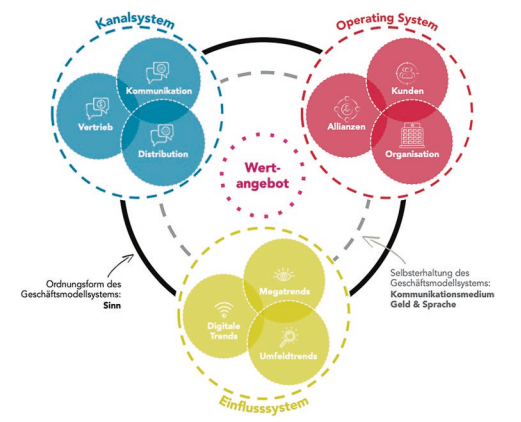
\includegraphics[width=\linewidth]{images/business-model-system.png}
\label{fig:businessModelSystem}
\end{figure}



%
%	Theorieteil
%

\pagebreak
\section{Digitales Live Studium}

\onehalfspacing

\subsection{Traditional Distance Learning}

Traditional Distance Learning

\subsection{DLS Lectures}

DLS Lectures

\subsection{DLS Exams}

DLS Exams

\subsection{DLS Exams}

DLS Exams

\subsection{DLS Studio}

DLS Studio


%
%	Praxisbezug
%

\pagebreak
\section{Market Relevance}

\onehalfspacing

\subsection{Enrollment Figures}

Enrollment Figures

\subsection{Competition}

Competition

\subsection{Hybrid Models}

Hybrid Models

\subsection{Market Saturation}

Market Saturation


%
%	Fazit
%

\pagebreak
\section{Summary}

\onehalfspacing

The Digital Live Studium addresses the needs of students who cannot attend lectures in person, for personal reasons or because of location. Especially for people tied up in care work, the ability to participate in a live lecture without leaving home is a big plus.

Other players in the secondary education market have also embraced the idea, further validating the innovation and its usefulness.

We can conclude that DLS is a highly successful innovation by FOM, and it will help the university stay competitive in the tight education market.

A further enhancement could be allowing the lecturers to work from home or their personal office.

Happy teaching!


%
%	Tools (Sopron)
%

\pagebreak
\section*{Tools}

\pagenumbering{gobble} % Keine Seitenzahlen mehr

\onehalfspacing

In addition to the documented references, these tools were used in creating this paper:

\begin{itemize}
    \item \href{http://www.overleaf.com}{Overleaf} to write the LaTeX source code
    \item \href{https://github.com/chfrank-cgn}{GitHub} for backup and version control
    \item Anthropic's \href{https://www.anthropic.com/claude}{Claude} for research
    \item \href{https://app.grammarly.com/}{Grammarly} for spellcheck and style
\end{itemize}


% Literaturverzeichnis
\cleardoublepage
\raggedright
\bibliographystyle{IEEEtranS}	% ieeetran verwenden, damit auch URLs angezeigt werden
\bibliography{seminar-lit}

\cleardoublepage
\justify
%
%	Ehrenwoertliche Erklaerung
%

\pagebreak

\pagenumbering{gobble} % Keine Seitenzahlen mehr
\onehalfspacing

%-----------------------------------
% Ehrenwoertliche Erklärung
%-----------------------------------
\section*{Declaration in lieu of oath}

\par\medskip

With this, I declare that I produced the submitted paper independently, without assistance from any other party, and without using any unauthorized aids. In particular, I have marked all passages reproduced verbatim or near-verbatim from publications as quotations. Also, I declare that the submitted print version of this thesis is identical to its digital version. Furthermore, I have never presented this thesis to any examination board in its current form or any other similar version. I herewith agree that you may publish this thesis. I hereby consent to you uploading this thesis to an external contractor's server for submission to their plagiarism detection systems. Uploading this thesis to send it to plagiarism detection systems does not constitute publication.

\par\medskip
\par\medskip

\vspace{5cm}

\begin{table}[H]
	\begin{tabular*}{\textwidth}{c @{\extracolsep{\fill}} ccccc}
		Cologne, \the\month/\the\day/\the\year \\
		\rule[0.5ex]{12em}{0.55pt} & \rule[0.5ex]{12em}{0.55pt} \\
		(Location, Date) & (Signature)
	\end{tabular*}
\end{table}


\end{document}
